\documentclass[a4paper, amsfonts, amssymb, amsmath, reprint, showkeys, nofootinbib, twoside]{revtex4-1}
\usepackage[english]{babel}
\usepackage[utf8]{inputenc}
\usepackage[colorinlistoftodos, color=green!40, prependcaption]{todonotes}
\usepackage[pdftex, pdftitle={Article}, pdfauthor={Author}]{hyperref}
\usepackage{amsthm}
\usepackage{mathtools}
\usepackage{physics}
\usepackage{xcolor}
\usepackage{caption}
\usepackage{hyperref}
%\hypersetup{colorlinks=true, linkcolor=blue, urlcolor = blue}
\usepackage{amsmath}
\usepackage{amssymb}
\usepackage{graphicx}
\graphicspath{Images}
\usepackage[left=23mm,right=13mm,top=35mm,columnsep=15pt]{geometry} 
\usepackage{adjustbox}
\usepackage{placeins}
\usepackage[T1]{fontenc}
\usepackage{float}
%\usepackage{longtable}
\usepackage{csquotes}
\usepackage{refstyle}
\usepackage{lipsum}
\usepackage{booktabs}



\begin{document}

\title{Study of Diffraction and Interference through single slit and double slits.}
\author{Swaroop Ramakant Avarsekar}
\email{swaroop.avarsekar@niser.ac.in}
\affiliation{School of Physical Sciences, National Institute of Science Education and Research, HBNI, Jatni -752050, India}
\date{\today}
	
\maketitle

\section{Introduction and Theory}
The wave nature of light was explained by Huygen, Frensel. When wave passes through a slit, different portions of emerging wavefront with travel in different distances before reaching screen. Here, the diffraction is studied and experimented under Fraunhofer regime. In the Fraunhofer, 
\begin{equation}
	I\propto \frac{sin^2\mu}{\mu^2}. cos^2\gamma
\end{equation}
 where $\beta=\pi b sin \theta/\lambda$ and $\gamma=\pi d sin \theta/\lambda$, d=b+c
 
 The first term of RHS represents diffraction pattern produced by single-slit and second term is characteristic of interference with phase difference $\gamma$. 

The positions of minima in single slit diffraction is given by
\begin{equation}
	bsin\theta=n\lambda; n=\pm1,\pm2....
\end{equation}
 If $\theta$ is small (screen distance is large compared to distance $x_m$ between two minima on either side of principal maximum), 
 \begin{equation}
 	sin\theta \approx \theta=\frac{x_m}{2D} \implies m\lambda=b\frac{x_m}{2D} 
 \end{equation}
Above equation can be used to determine the wavelength of monochromatic light. 

\begin{figure}[htbp] %  figure placement: here, top, bottom, or page
	\centering
	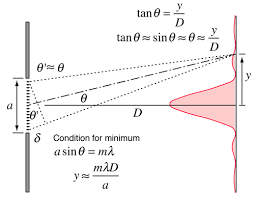
\includegraphics[width=8cm]{5} 
	\caption{Single slit intensity}
	\label{1}
\end{figure}

The thin wire also leads a diffraction pattern on screen identical to that of slit. To determine the thickness of the wire b, 

\begin{equation}
	b= 2m\lambda D/x_m
\end{equation}

Babinet's principle - The diffraction pattern from and opaque body (wire) is same as that of slit of same size and shape except the central maxima. 

\begin{figure}[htbp] %  figure placement: here, top, bottom, or page
	\centering
	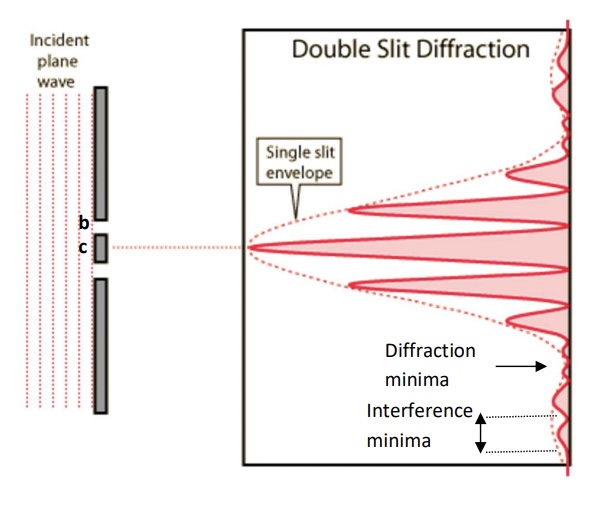
\includegraphics[width=8cm]{6} 
	\caption{Double slit intensity}
\end{figure}

The minima conditions for interference are,
\begin{equation}
	d sin\theta= (p+1/2)\lambda
\end{equation}

From the conditions for diffraction and interference, we can determine the slit width and separation as,
\begin{equation}
	b= n\lambda D/\Delta x_m
\end{equation}

\begin{equation}
	d= n\lambda D/\Delta x_p
\end{equation}

$\Delta x_p$=Distance between successive interference minima and $\Delta x_m$=Distance between successive interference minima .

\section{Experiment}
\subsection{Apparatus}
The experimental setup consists of single and double slits, and thin wire, with laser as light source. The graph papered screen is placed few meters away from the slit. The measuring tape is used to measure distance. Traveling microscope will be used to measure the slit and wire thickness. The laser along with height adjustment setup is required.  
\subsection{Procedure}
Determine the vernier constant to traveling microscope and measure thickness of wire, single slit, double slit and slit + wire of double slit. Place the screen meters apart from slit, where screen is attached with graph paper. Turn on the laser with and adjust the height of it according to the single  slit placed on the optical bench. Adjust the slit width so that the diffraction pattern is crisp and atleast few order patterns are visible on the screen. Mark the intensity patterns with pencil, preferably the minima. Measure the screen distance by using tape.. The same is repeated with thin wire and double slits. Babinet's principle can verified keeping the wire and slit in front of each other. With the double slits, we can also observe interference pattern along with diffraction pattern.

\begin{figure}[htbp] %  figure placement: here, top, bottom, or page
	\centering
	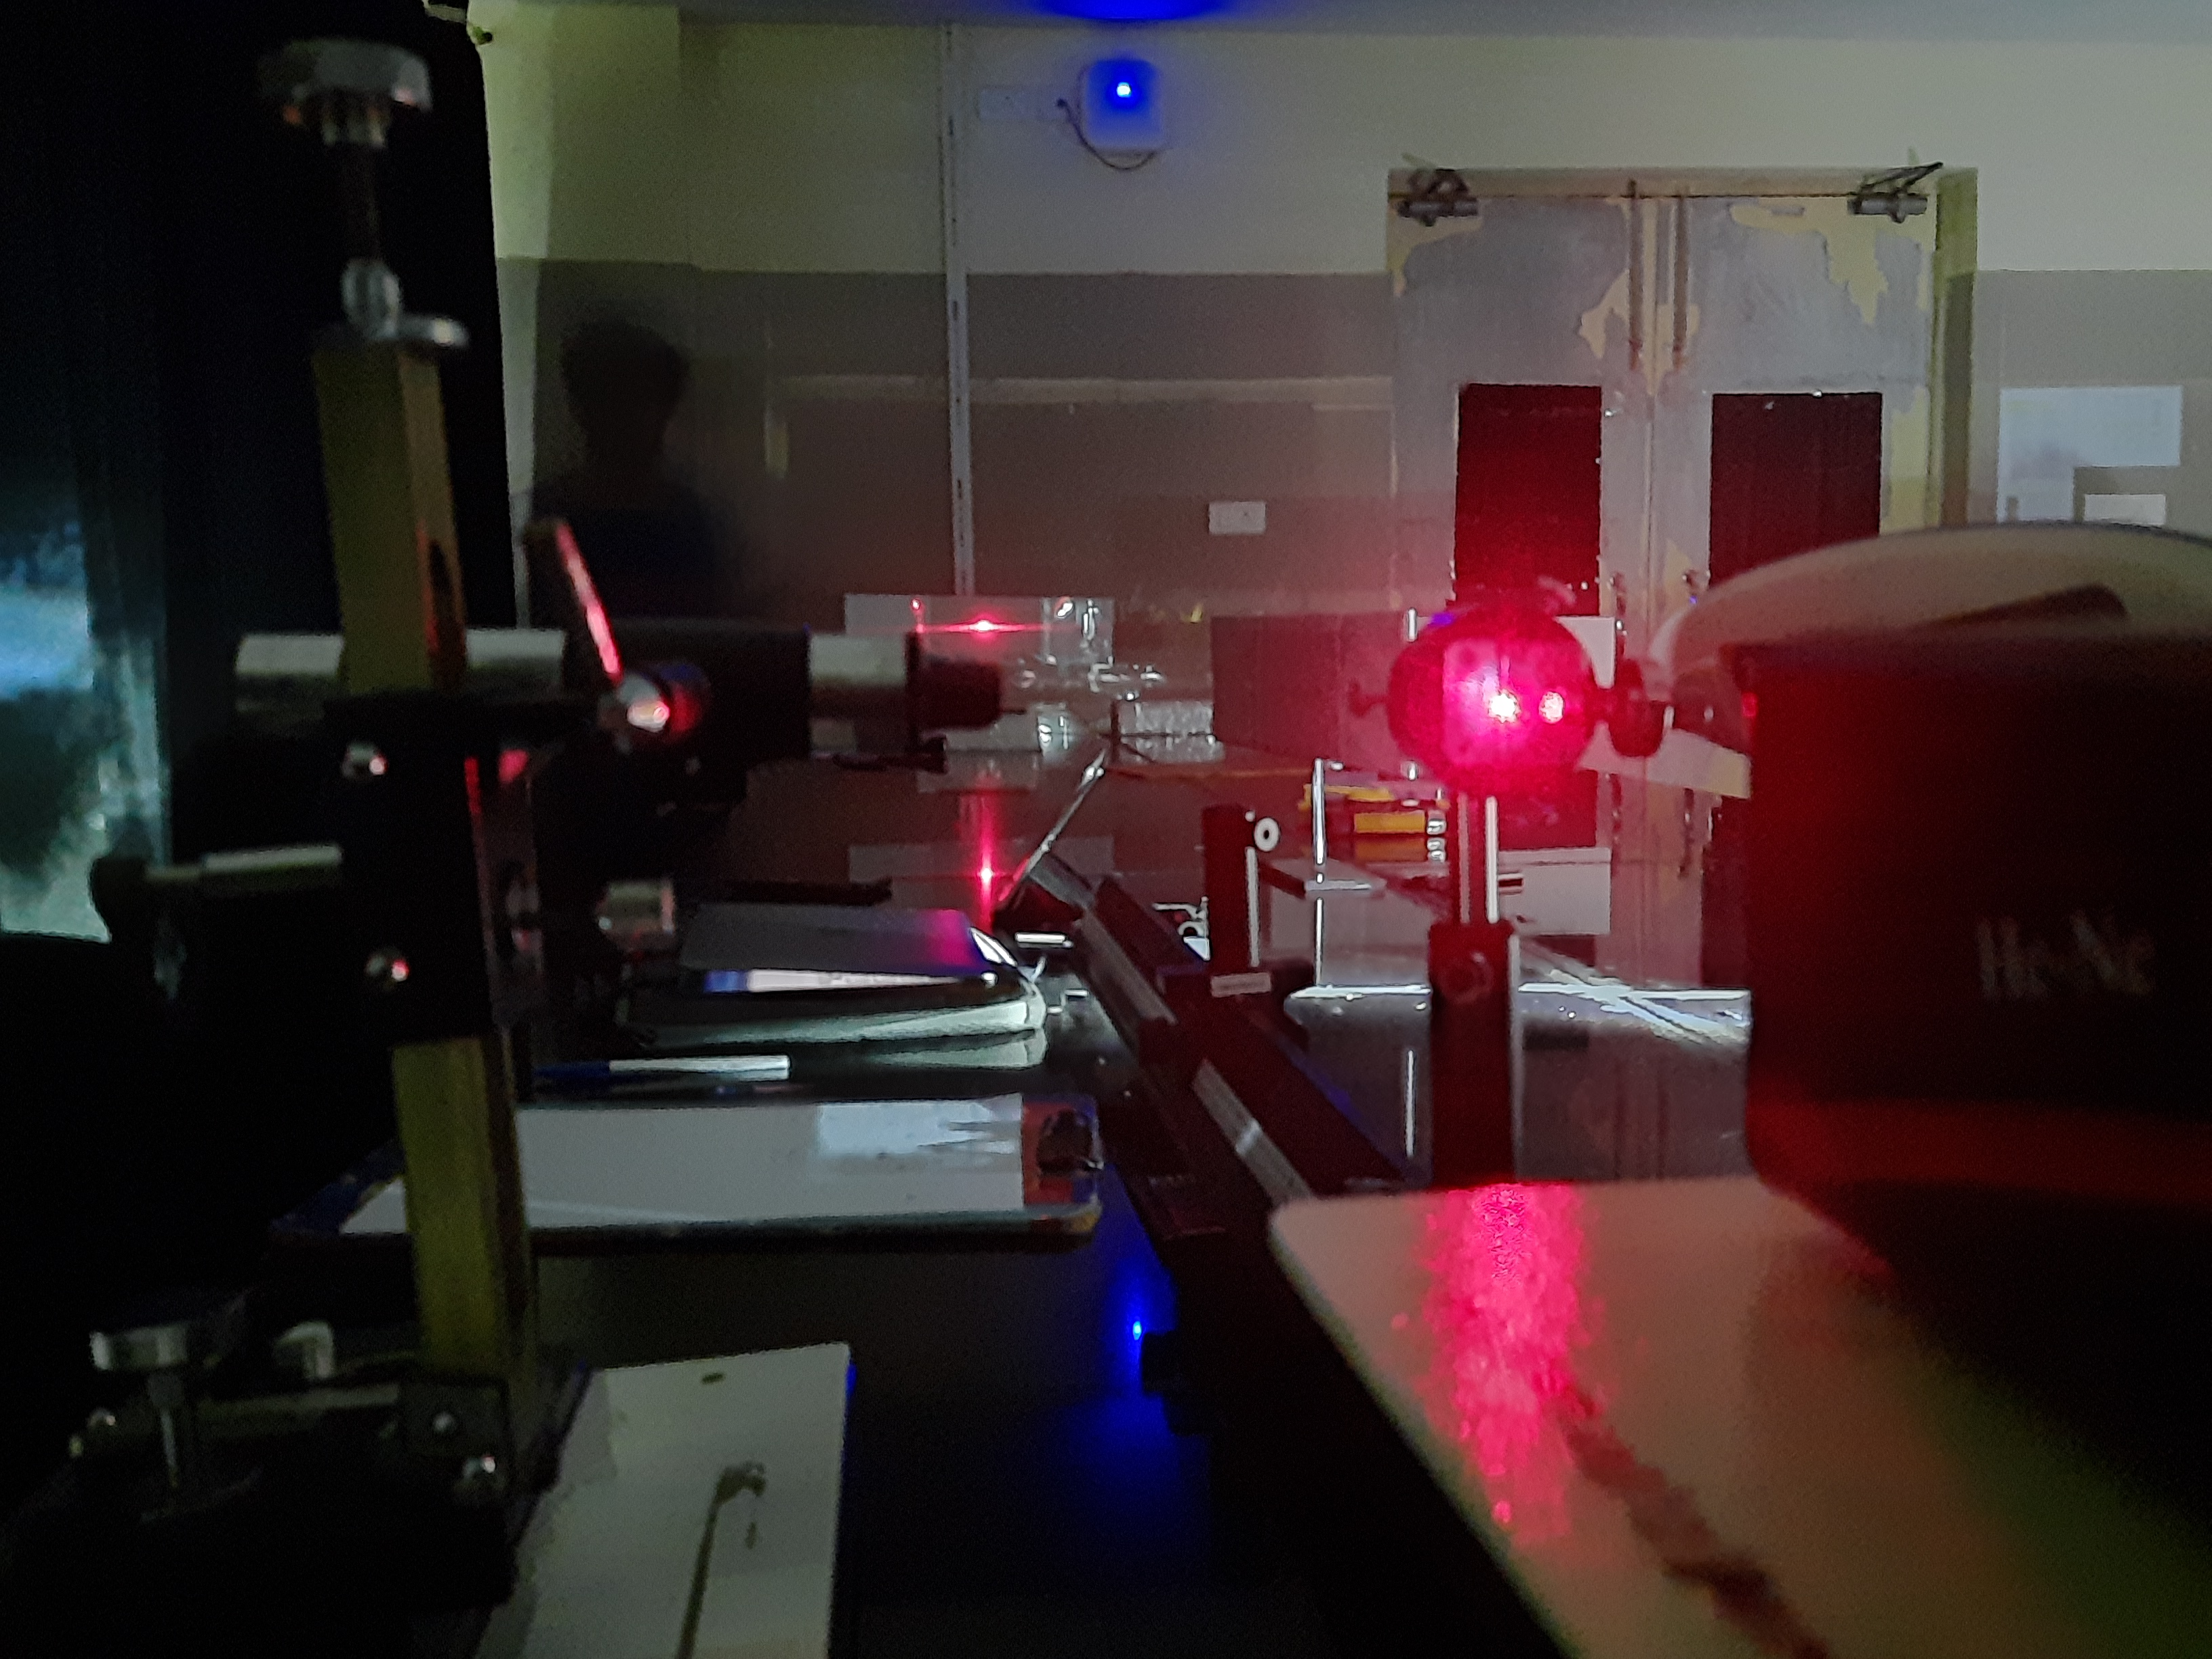
\includegraphics[width=8cm]{1} 
	\caption{Experimental setup in laboratory}
\end{figure}

\subsection{Precautions}
\begin{enumerate}
\item{Make sure the screw of slits are tight enough so that the intensity pattern does not change.}
\item{Never make direct eye contact with the laser beam.}
\item{Use of safety goggles is advisable.}
\end{enumerate}

\subsection{Observations and Analysis}

\begin{figure}[H] %  figure placement: here, top, bottom, or page
	\centering
	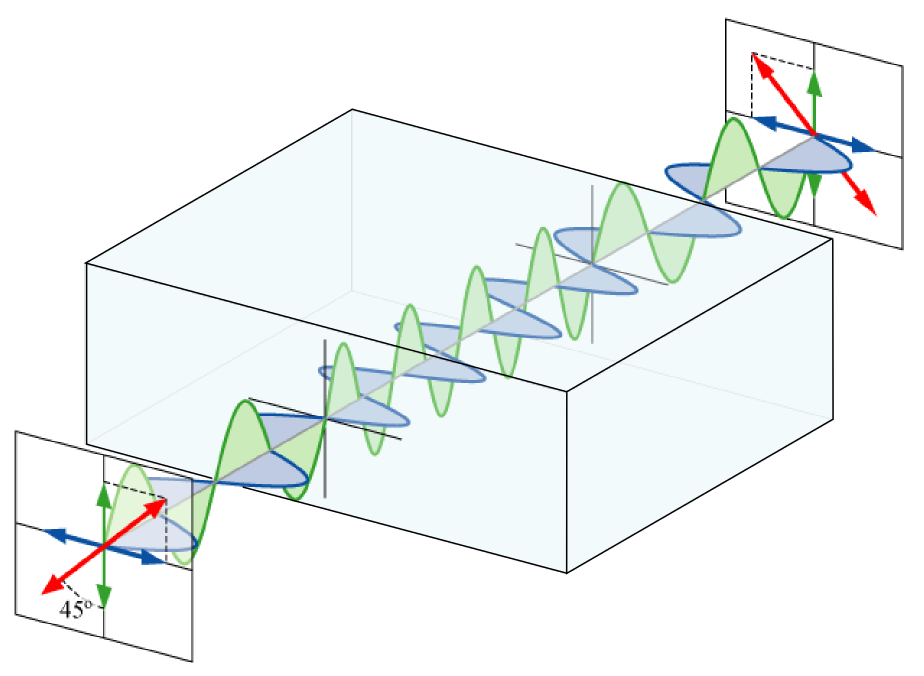
\includegraphics[width=8cm]{2} 
	\caption{Single slit diffraction pattern}
\end{figure}

\begin{figure}[H] %  figure placement: here, top, bottom, or page
	\centering
	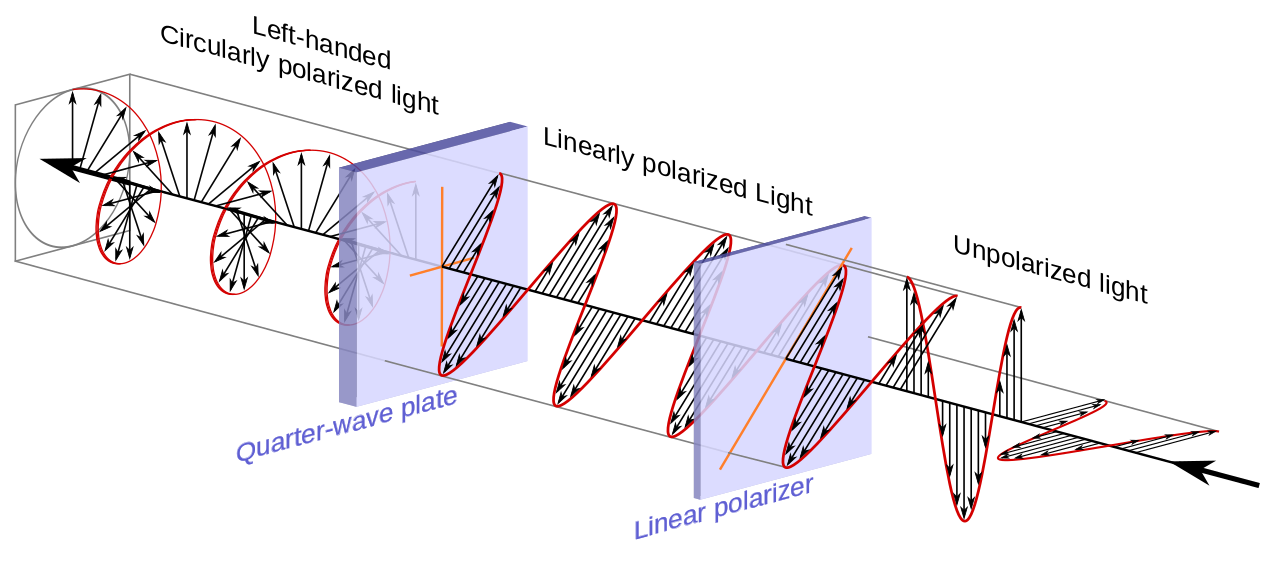
\includegraphics[width=8cm]{3} 
	\caption{Thin wire diffraction pattern}
\end{figure}

\begin{figure}[H] %  figure placement: here, top, bottom, or page
	\centering
	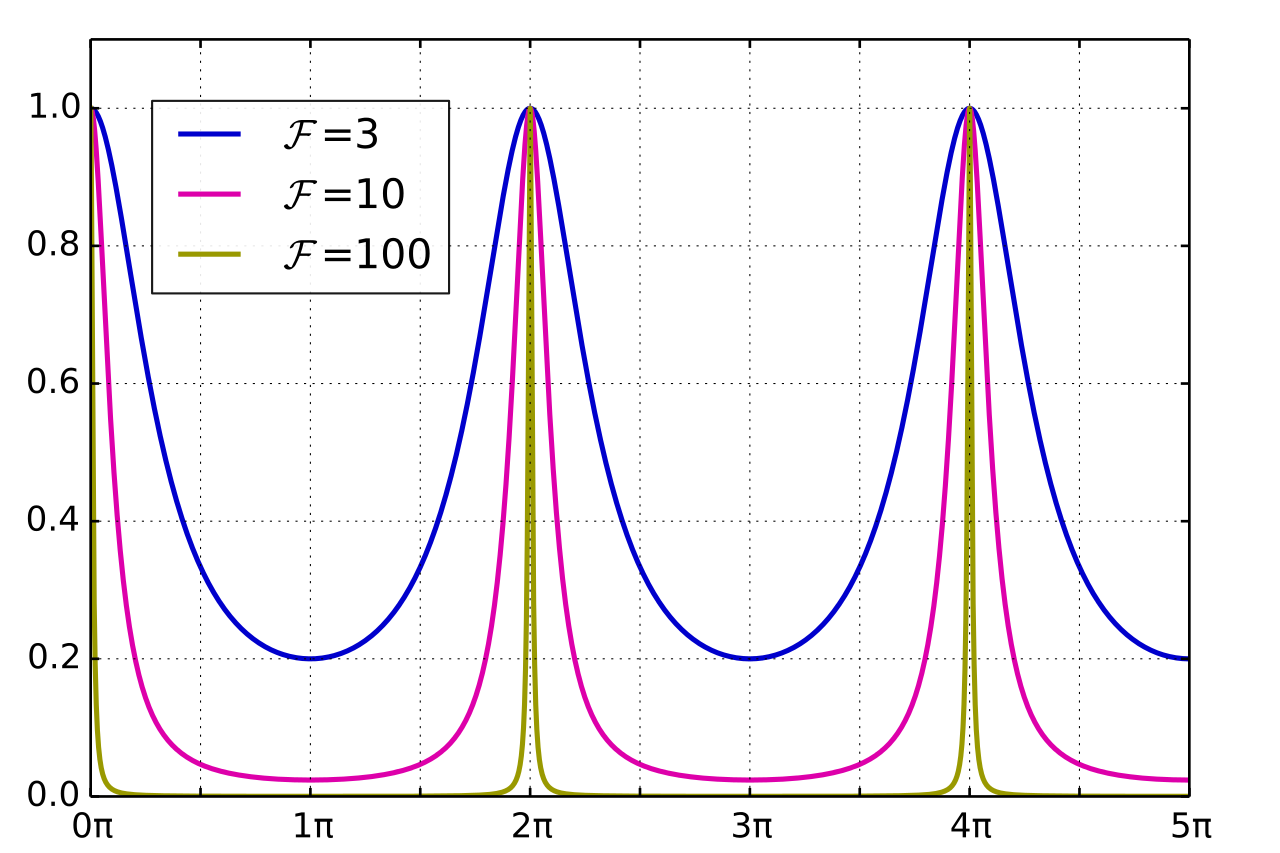
\includegraphics[width=8cm]{4} 
	\caption{Double slit diffraction and interference pattern}
\end{figure}

\begin{figure}[H] %  figure placement: here, top, bottom, or page
	\centering
	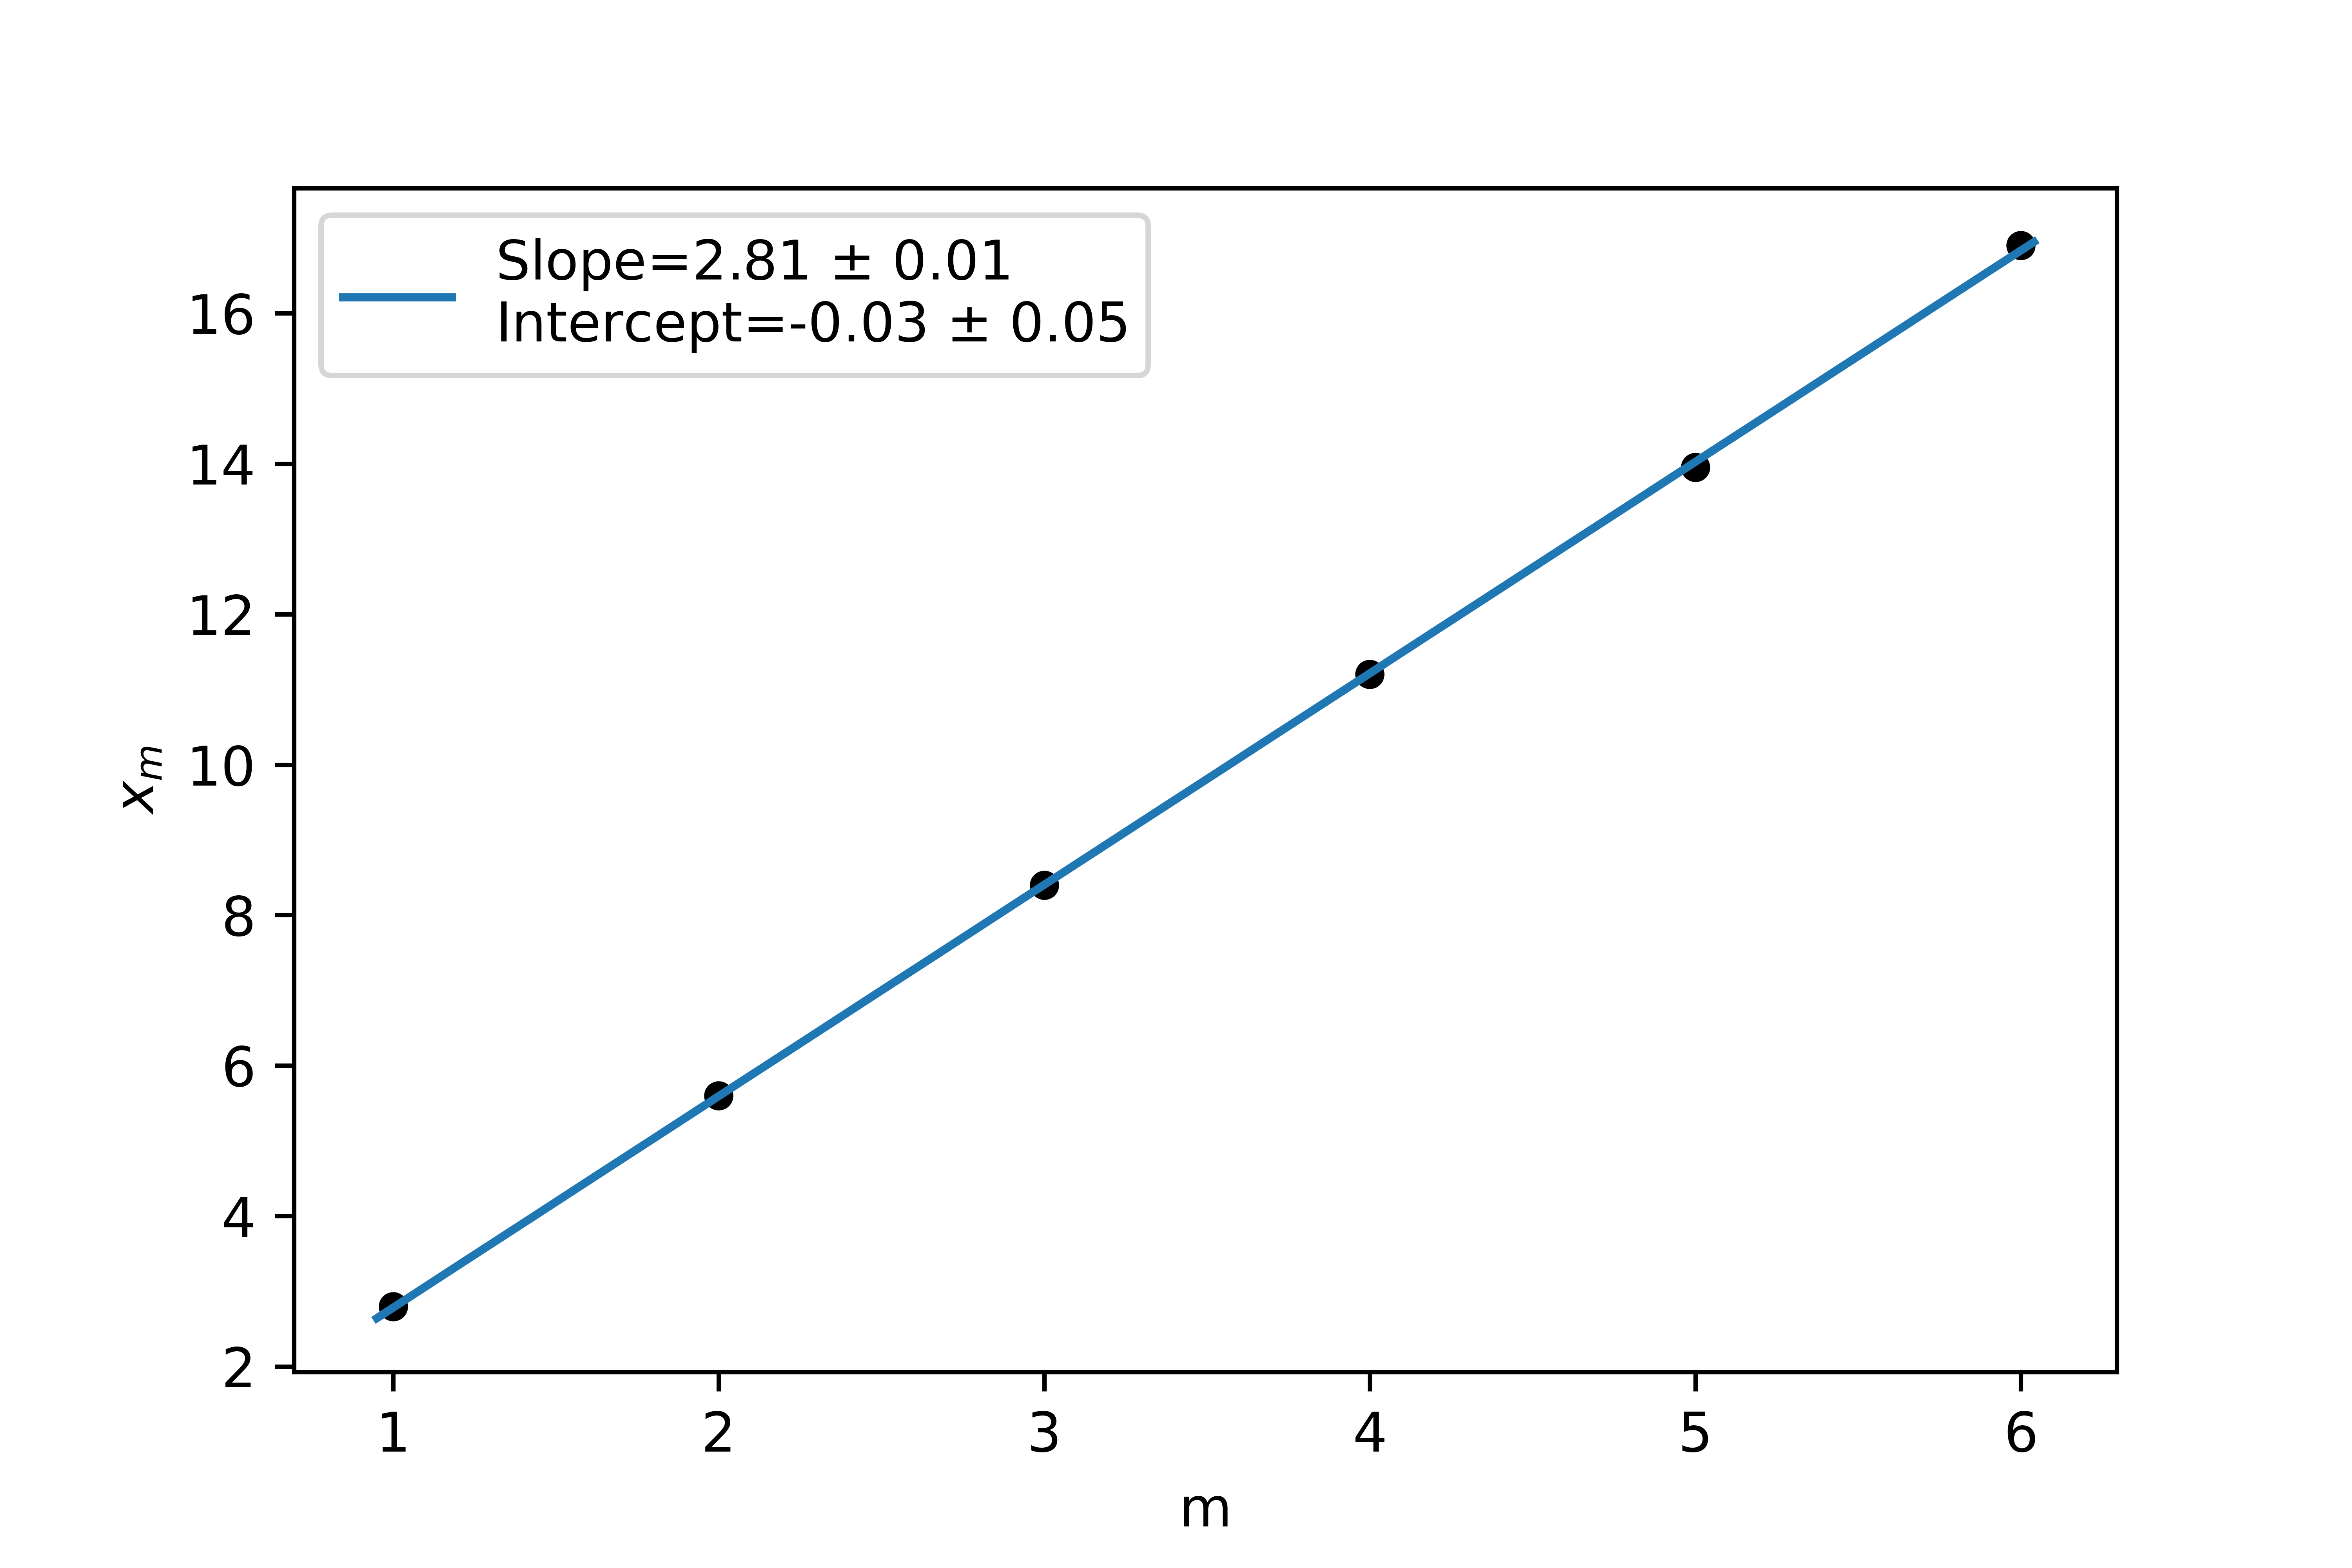
\includegraphics[width=8cm]{p1} 
	\caption{Single slit-Plot of order v/s distance of minima}
\end{figure}

The slope of linear fit is $2.81\pm0.01$ cm. Therefore, from equation (3), we calculate $\lambda$,
\begin{equation}
	\lambda=Slope. b/2D= 989.88 nm
\end{equation}

Error in $\lambda$,
\begin{equation}
\delta \lambda=\lambda \left(\sqrt{\left(\frac{\delta b}{b}\right)^2+\left(\frac{\delta Slope}{Slope}\right)^2}\right)
\end{equation}

\begin{equation}
	\delta \lambda=989.88 \left(\sqrt{\left(\frac{0.008}{0.031}\right)^2+\left(\frac{0.01}{2.81}\right)^2}\right)=255.46 nm
\end{equation}

From equation (4), we can determine the thickness of wire with known $\lambda$ ,

\begin{figure}[H] %  figure placement: here, top, bottom, or page
	\centering
	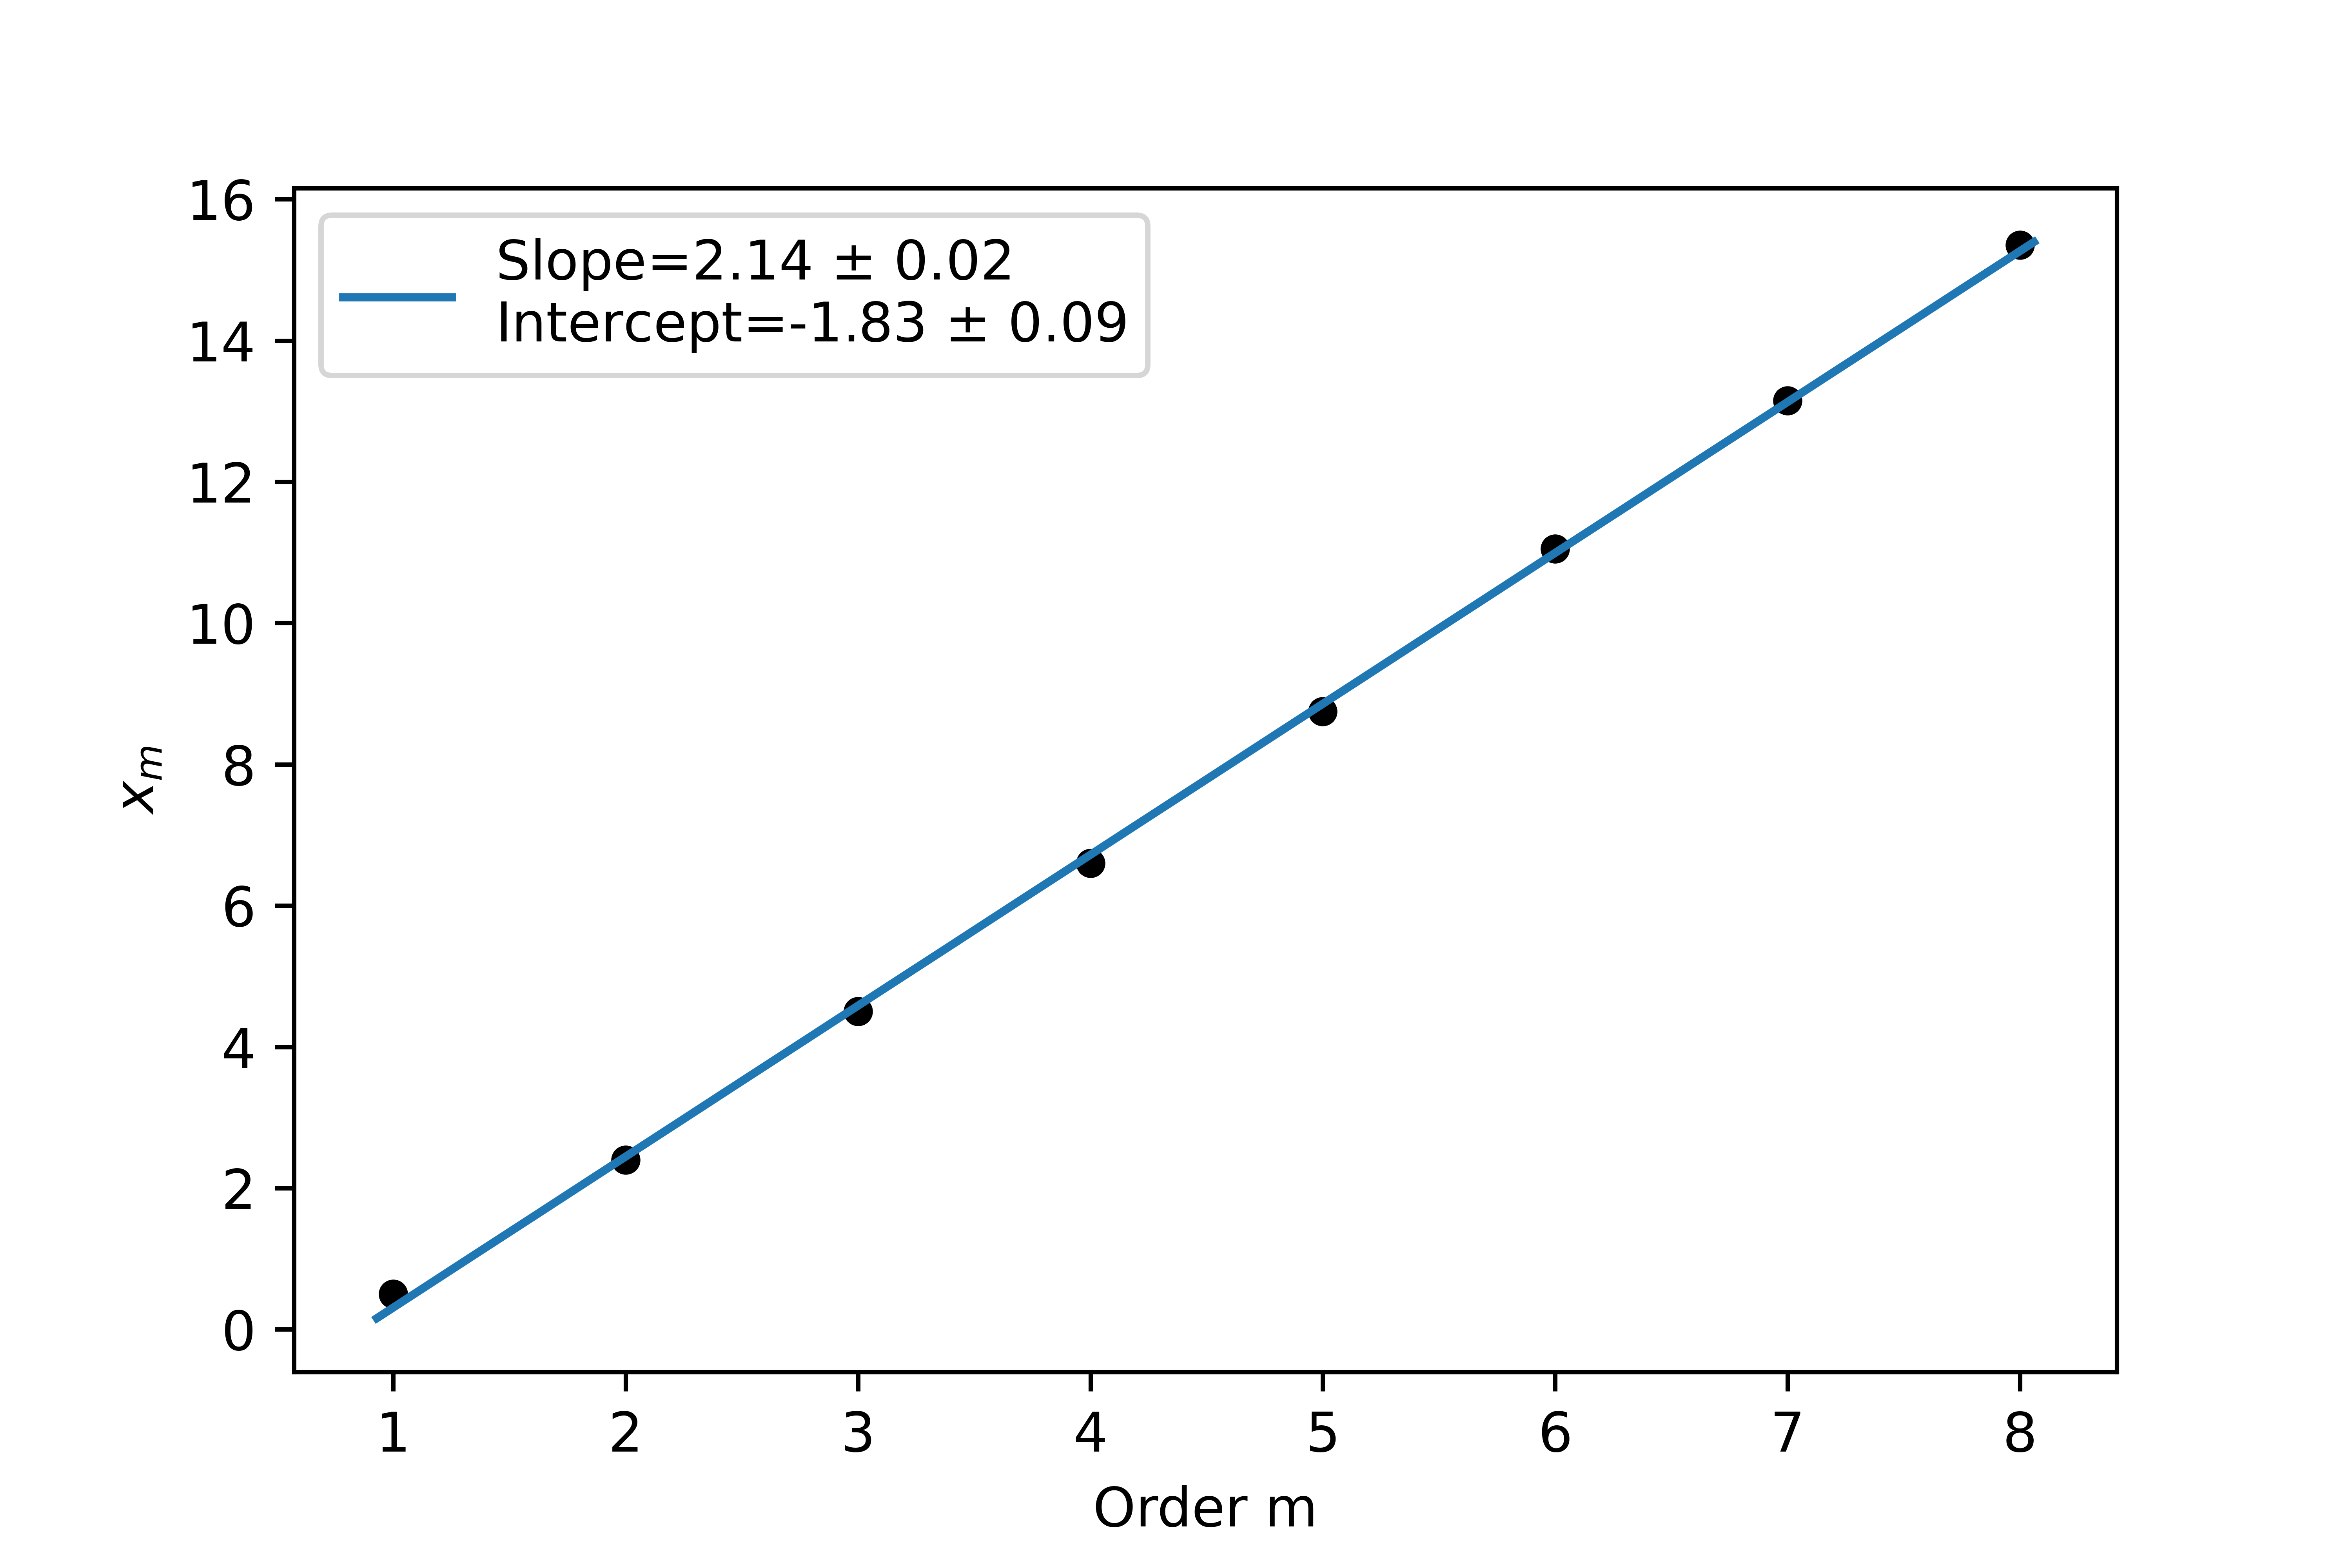
\includegraphics[width=8cm]{p2} 
	\caption{Thin wire -Plot of order v/s distance of minima}
\end{figure}

Equation (4) can be modified as
\begin{equation}
	b=2.\lambda. D/Slope
\end{equation}

From the plot, Figure (8) we get wire thickness as b=0.032 cm

Error in b is,
\begin{equation}
	\delta b=b \left(\sqrt{\left(\frac{\delta \lambda}{\lambda}\right)^2+\left(\frac{\delta D}{D}\right)^2+\left(\frac{\delta Slope}{Slope}\right)^2}\right)
\end{equation}

Giving $\delta b$=0.008 cm
 
Error analysis for b from Table 4,
\begin{equation}
	\delta b=b \left(\sqrt{\left(\frac{\delta \lambda}{\lambda}\right)^2+\left(\frac{\delta D}{D}\right)^2+\left(\frac{\delta x_m}{x_m}\right)^2}\right)
\end{equation}

Giving $\delta b$=0.002 cm

From the observations from table 3 and table 4, we get b=$0.032\pm0.008$ cm and b=$0.032\pm0.002$ cm. Comparing these two values of b, Babinet's principle is verified that the slit width and wire thickness is same, resulting identical fringe pattern.

From the Table 5 and 6, error in c is calculated as 
\begin{equation}
	\delta c=\sqrt{(\delta d)^2+(\delta b)^2}
\end{equation}

$(\delta d)$ and $(\delta b)$ are least count of the instrument. Therefore, we obtain $(\delta c)$=0.001 cm

From, table 5 and table 6, we obtained the opaque distance between two slits as $0.017\pm0.001$ cm and $0.023\pm0.001$. 

\section{Conclusion}
From this experiment we found out the wavelength of light used as $(989.88\pm255.46)$ nm which deviates from the literature value of He-Ne laser light. The width of single slit and wire calculated from travelling microscope is $0.031\pm0.001$ cm and $0.020\pm0.001$ cm. We also verified Babinet's principle and found that the thin wire and single slit of same thickness produce same diffraction pattern. We obtained thickness of slit and wire as b=$0.032\pm0.008$ cm and b=$0.032\pm0.002$ cm respectively. We also calculated the opaque distance between two slits as $0.017\pm0.001$ cm and $0.023\pm0.001$ cm. 

We see that the errors are resulted due to traveling microscope, such as backlash error. The wavelength obtained from the experiment is very high. The markings on the screen also contributes to the error in calculation of wavelength. Some human errors and random errors have propped up while doing the experiment as they were performed in two different days probably with different apparatus. The value could be improved by taking more readings, but it was hindered due to the time constraints to setup and perform the experiment.

\section{References}
\begin{enumerate}
\item{\url{https://www.niser.ac.in/sps/sites/default/files/basic_page/Diffraction%20of%20laser%20light%20using%20various%20apertures.pdf}}
\item{\url{http://hyperphysics.phy-astr.gsu.edu/hbase/phyopt/sinslit.html}}
\item{\url{https://en.wikipedia.org/wiki/Babinet%27s_principle}}
\end{enumerate}
\end{document}